%=====================================================================
\chapter{Latexbefehle beispielhaft erkl�rt}
\label{sec:latexbeispielkapitel}
%=====================================================================
Die folgenden Beispielbefehle sollen den Umgang mit Latex erleichtern.
\section{Tabellen einf�gen}
Tabellen k�nnen ohne weiteres eingef�gt werden.
\begin{table}[h!]
  \centering
  \caption{Geometrische Grenzen f�r t1}
\begin{scriptsize}
    \begin{tabular}{rc|c}
    %\toprule
          &       & gegebene Werte\\
    \hline
    Rotordurchmesser & $[m]$ & 1 \\
    Max. H�he von Bauwerk & $[m]$ & 1 \\
    Max. Breite von Bauwerk  & [m]   & 2.00 \\
    Saugrohrl�nge & [m]   & Optimierte Leistung \\
    \hline
    %\bottomrule
    \end{tabular}%
  \end{scriptsize}
  \label{tab:geom_boundaries_t1}%
\end{table}%
Hierbei zeigt~\ref{tab:geom_boundaries_t1} eine richtige Referenz im Text. Tabellen, die eingef�gt werden, m�ssen immer im Text referenziert werden.
\section{Graphen einf�gen}
Der Beispielgraph~\ref{abb:pvsrpm} mit der Referenz ist richtig eingef�gt.
\begin{figure}[h!]
 \includegraphics[scale=0.6,angle=-90]{pics/leistungdrehzahlt1.eps}
\caption{Leistung �ber Drehzahl von Turbine t1 f�r verschiedene Anstr�mgeschwindigkeiten}
\label{abb:pvsrpm}
\end{figure} 
Eingef�gte Bilder und Graphen m�ssen immer im Text eindeutig referenziert werden.
\section{Literaturverweise}
Literaturquellen m�ssen immer vollst�ndig angegeben und referenziert werden, wie z.B.~\cite{ansys1}. Hierbei nimmt Latex die Sortierung automatisch vor. Die Eintr�ge werden in der Datei ``literatur.bib'' eingef�gt.
\section{Die mathematische Umgebung}
Des Weiteren k�nnen Abk�rzungen mittels der mathematische Umgebung, z.B. so $3 m/s$ eingef�gt werden.
Die Formel im Text $v=\frac{s}{t}$ ist g�ltig.
Die folgende Formel
\begin{equation}
        v=\frac{s}{t}
\label{equ:geschwindigkeitlinear}
\end{equation} 
ist nummeriert. Ein Verweis ist m�glich, weil die Formel~\ref{equ:geschwindigkeitlinear} ein Label hat.
\section{Abk�rzungen}
Abk�rzungen m�ssen wie auch Konstanten und Indizes in der Nomenklatur alphabetisch aufgef�hrt werden. Die Datei ``nomenklatur1.tex'' enth�lt viele Beispiele, die n�tzlich sein k�nnen\footnote{Die Datei liegt dem Ordner bei. Zudem zeigt die Fu�note, wie diese verwendet werden kann}.
